\section{Auswertung}
\label{sec:auswertung}

Zu Beginn wurden aus den zur Verf\"ugung gestellten Datens\"atzen alle Attribute die Monte Carlo Daten, Gewichte und Labels enthalten, entfernt. Au\ss erdem wurden die Spalten entfernt, die ausschlie\ss lich den selben Wert, "Inf" oder "not a Number" enthalten.
Die Spalten wurden komplett entfernt damit ausschlie\ss lich vollst\"andige Attribute verwendet werden.
Wie in Tabelle \ref{tab:results} zusehen ist, sind die Effizienzen trotzdem sehr gut.
Abschlie\ss end wurden Signal und Hintergrund Samples auf Attribute \"uberpr\"uft, die nur in einem der beiden Samples auftreten und diese ebenfalls entfernt. Dadurch wurden zwei Datens\"atze mit identischen Attributen erzeugt.
Um sp\"ater zwischen Hintergrund und Signal unterscheiden zu k\"onnen, wurde an das Signal mit "0" gelabelt und der Hintergrund mit "1".

Im Folgenden werden wir drei verschieden Klassifizierer auf eine Auswahl an Attributen testen. Es werden der \texttt{Naive-Bayes} Klassifizierer, der \texttt{RandomForestClassifier} und der \texttt{KNeighborsClassifier} mit Hilfe von \texttt{sklearn} verwendet.
Zun\"achst wurde die beste Anzahl an Attributen ermittelt indem Anhand des \texttt{KNeighborsClassifier} der Jaccard Score in Abh\"angigkeit der Attributsanzahl bestimmt wurde. Dies resultiert darin, dass bei 50 Attributen der gr\"o\ss te Jaccard Score auftritt.
F\"ur alle weiteren Analyseschritte wurden also die besten 50 Attribute, ermittelt mit der \texttt{SelectKBest} Methode, verwendet.
Die G\"ute der Attribute wurde mit dem \texttt{f\_classif} ermittelt.
Aus diesen Attributen wurden Test- und Trainingsdatens\"atze extrahiert, mit welchen die obigen Klassifizierer nun getestet werden.

Zuerst wurde der \texttt{RandomForestClassifier} verwendet.
Dafür wurde ein \texttt{RandomForest} mit 100 Entscheidungsb\"aumen gew\"ahlt\footnote{100 Entscheidungsb\"aume sind auch die default Einstellung. Mehr B\"aume erzielen keine h\"ohere Effizienz}. Alle anderen Parameter wurde mit default initialisiert.
Mit der Vorhersage des Klassifizierers wurden die Effizienz und die Reinheit bestimmt.
Au\ss erdem wurde der Jaccard Score f\"ur unsere obige Attributsauswahl berechnet. Die entsprechende ROC-Kurve ist Abbildung \ref{fig:roc_curves} zu entnehmen.
Die Ergebnisse stehen in Tabelle \ref{tab:results}.

F\"ur den \texttt{KNeighborsClassifier} wurden 20 Nachbarn gew\"ahlt.
Es l\"asst sich zeigen, dass die Anzahl an n\"achsten Nachbarn nicht von Relevanz ist, wenn mindestens 20 Nachbarn gew\"ahlt werden.
Auch hier wird die Vorhersage und der Jaccard Score in Tabelle \ref{tab:results} dargestellt sowie die ROC-Kurve in Abbildung \ref{fig:roc_curves}.

Zuletzt wurde der Naive-Bayes Klassifizierer, welcher dem Prinzip der bedingten Wahrscheinlichkeiten gen\"ugt, getestet.
Die Ergebnisse befinden sich wieder in Tabelle \ref{tab:results} und der Abbildung \ref{fig:roc_curves}.

% RandomForest
% Effizienz: 0.9770 (+/- 0.0052)
% Reinheit: 0.9556 (+/- 0.0060)
% Jaccard Index: 0.9351 (+/- 0.0024)
%
% kNN
% Effizienz: 0.7421 (+/- 0.0072)
% Reinheit: 0.7421 (+/- 0.0065)
% Jaccard Index: 0.7421 (+/- 0.0041)
%
% naive bayes
% Effizienz: 0.8080 (+/- 0.0283)
% Reinheit: 0.8014 (+/- 0.0142)
% Jaccard Index: 0.6730 (+/- 0.0112)

\begin{table}
  \centering
  \begin{tabular}{c | c c c}
    \toprule
    \text{Klassifizierer} & \text{Effizienz} & \text{Reinheit} & \text{Jaccard Score} \\
    \midrule
    \text{RandomForest} & $\num{0.9770(0052)}$ & $\num{0.9556(0060)}$ & $\num{0.9351(0024)}$ \\
    \text{KNeighborsClassifier} & $\num{0.7421(0072)}$ & $\num{0.7421(0065)}$ & $\num{0.7421(0041)}$ \\
    \text{Naive-Bayes} & $\num{0.8080(0283)}$ & $\num{0.8014(0142)}$ & $\num{0.6730(0112)}$ \\
    \bottomrule
  \end{tabular}
  \caption{Effizienz, Reinheit und Jaccard Score der drei verwendeten Klassifizierer.}
  \label{tab:results}
\end{table}

\begin{figure}
  \centering
  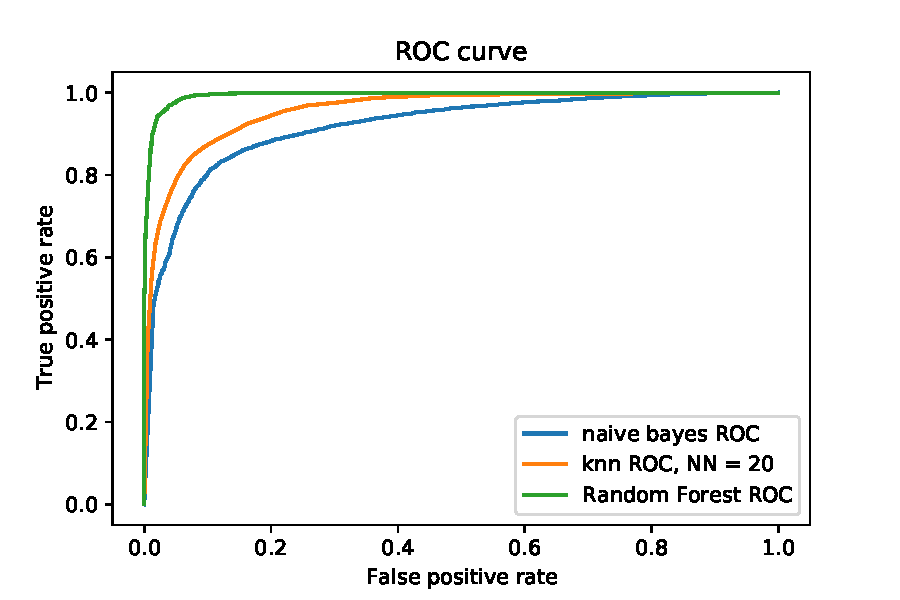
\includegraphics[width=0.8\textwidth]{plots/roc_curve.pdf}
  \caption{ROC-Kurven aller getesteten Klassifizierer.}
  \label{fig:roc_curves}
\end{figure}
